\chapter{Data Acquisition (DAQ)}
 
\section{Introduction}

In order to measure data from the experiment that can be analyzed, visualized and manipulated it is necessary to sample signals from sensors and convert them digital numeric values. This process is called data acquisition (DAQ) and can be achieved by various different software programs and a variety of general purpose programming languages. In general it can be differed in source, DAQ hardware and DAQ software. Whereas the source represents the sensor and measures the physical property, e.g. temperature, current, and magnetic flux density, DAQ hardware is usually the interface between the signal and the PC. Components like analog/digital converters, multiplexer, RAM etc. are common on this level. Microcontrollers, on which small programs run, can access those hardware devices via a bus and a protocol to make them available for further usage. DAQ software is necessary to make the DAQ hardware to communicate and work with a PC. While device drivers perform read and writes access at a very low-level on the hardware, standardized APIs \footnote{Application Programming Interfaces} enable a more abstract access and allow developing advanced user applications.\\

Data acquisition is an important part of the nEDM experiment since it is necessary to measure and store data from various sensors. Storing the data to make visualizing and analyzing possible afterwards is crucial to successfully run the experiment. There are lots of different aspects that need to be considered when setting up a new data acquisition system. To ensure a high quality system some basic requirements have to be met\cite{Schneider12, Marino12}:

\begin{itemize}
\item Expandability, to add a new subsystem
\item Adaptability, to handle different types of subsystems 
\item Security and Reliability, validation and backups to prevent data corruption
\item Layered Structure, to keep the system lucid and stable
\item Remote controllability, to have an easy access to the status of the experiment
\end{itemize}

\subsubsection*{Expandability}
Simple and modular implementation should lead to a system where new devices and subsystems are easily added. Adding additional devices should follow the "plug in and play" paradigm. No sophisticated implementation should be necessary when extending the system with new devices.

\subsubsection*{Adaptability}
Since subsystems can be implemented in a great variety of different controlling software and programming languages, e.g. LabVIEW, ORCA or python scripts, standardized interfaces are essential. Providing a fundamental application programming interface could meet this requirement and allows uncomplicated substitution of subsystems and devices. Furthermore adding devices to measure newly identified physical effects is getting easy.

\subsubsection*{Security and Reliability}
Encapsulation of used data storage should be possible. Different devices should be able to write on separate databases to avoid data loss or data corruption. Using this approach the risk decreases and different levels of accessibility can be set to prevent unauthorized access of the data. Furthermore continuous backup of all databases is required to prevent data loss caused by hardware failures or other errors. 

\subsubsection*{Layered Structure}
In software engineering the multi layer architecture is  common pattern to achieve logically separated functionality in a system. Functionality is implemented in independent modules that communicate with well defined interfaces. This very common model ensures a stable system, that is easy to understand and adapt. Data is stored on a database at the base layer. Separated from it a view/control layer is responsible to visualize and analyze the data.

\subsubsection*{Remote Controllability}
Watching the current experiments status should be possible and if necessary control devices from everywhere. Retrieving experimental data at a workstation in the laboratory, a PC at home or on a mobile device after authentication allows a remote access of the experiments status. Furthermore machine generated reports can automatically be send via mail to notify the project team of some extraordinary events or data.

\section{Data Acquisition Architecture}
\subsection{Multi-Tier Architectures}
A multi-tier architecture is common client-server architecture in which presentation, application processing, and data management funtions logically separated. Widely used thereby is the so called three-tier architecture. User interface, functional logic and data storage and access are developed and maintained as independent modules. This logical independence between the modules allows upgrades or changes without effecting the whole system. The usage of well-defined interfaces enables those separated evolve processes and therefore increases the agility and ability to meet upcoming requirements or changes.\\

Three-tier architectures consist of the following tiers:
 \begin{description}
     \item[Presentation tier] Visualizing data and interacting with the user are the most common services that are offered by the presentation tier. It retrieves data from the underlying data access tier and provides meaningful representations. This layer should furthermore be responsible for supplying user interfaces for devices accessing data, e.g. web browser at a PC or mobile device.
     \item[Application or data access tier] Data access tier is responsible for any business or data logic. Operations like selecting or aggregating data, as well as mathematical operations are performed within this layer. It expects data from the data tier and after executing necessary operations it serves the processed to the presentation tier according to the interfaces.
     \item[Data tier] This tier consists of the database storage. All data, that is measured by any sensor should be inserted and stored. Continuous backups as well as indexing and performance operations are kept at this level. The storage architecture itself should not be affected from any other tier.
  \end{description}
  
  
\begin{figure}[h!]
  \centering
      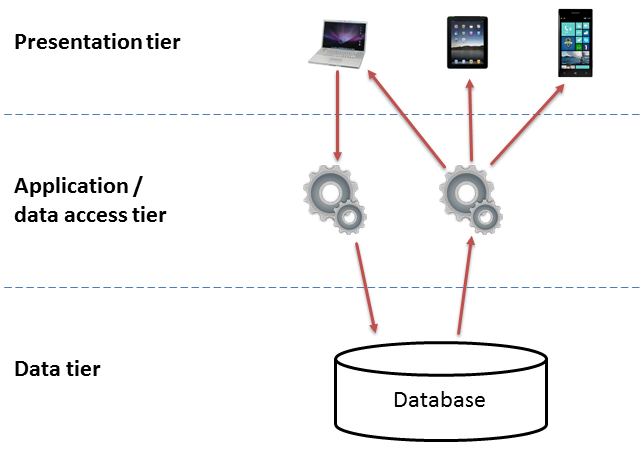
\includegraphics[width=0.7\textwidth]{images/3TierArchitecture.png}
  \caption{Schematic view of a three-tier architecture with one datastorage and different data representations using the data access level for information insertion and retrieval}
  \label{figure:3TierArchitecture}
\end{figure}

Figure \ref{figure:3TierArchitecture} shows an schematic overview of a three-tier architecture. A layer does only communicate with the tier that is directly below or above itself. The presentation layer does not call any functions from the database layer or vice versa.
  
\subsection{Data acquisition architecture at the nEDM experiment}
The three tier architecture is a very common pattern and used in many different software applications. Furthermore all patterns are best practices from a very abstract point of view. Therefore it is allowed to adapt this very general architectures to ones specific problem. Schneider showed the resulting architecture for the nEDM experiment in his bachelor thesis\cite{Schneider12}.\\

The architecture needs to provide three different layers to cover the requirements for the experiment. At the lowest level, there is a device layer that holds sensors measuring physical signals. Those signals are stored within a database, represented by a second layer. And the top layer is called View/Control layer and is responsible for providing views to the data and furthermore allows for controlling the database and physical devices via control parameters.
  
\begin{figure}[h!]
  \centering
      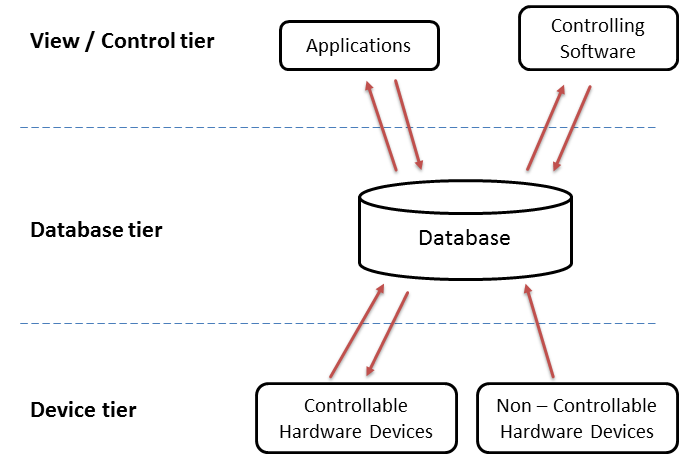
\includegraphics[width=0.7\textwidth]{images/DAQArchitecture.png}
  \caption{Adapted three tier architecture for the nEDM experiment}
  \label{figure:DAQArchitecture}
\end{figure}

Looking at the three tier architecture (see Figure \ref{figure:DAQArchitecture}) for the nEDM experiment more detailed, the following descriptions can be noted:
 \begin{description}
     \item[Device tier] The layer at the bottom is the hardware nearest layer. It consists of hardware controlling devices that are directly connected to all kinds of sensors. In general it can be differed between those sensors who can only send data to the database and those sensors that can furthermore also receive commands. 
     \item[Database tier] The database becomes the central part of the architecture. Beside its role as data storage it furthermore is responsible for the communication between the control applications and the hardware devices.  
     \item[View / Control tier] Although in standard three tier architectures the view layer is separated from the control layer, are those to tiers conflated to one. As we will see later on, the used technologies offer methods to combine the responsibilities of both layers. 
  \end{description}
  
  At this point a deviation from the standard pattern can be accepted because of the adaption to a very specific problem. Furthermore a best practice, recommended by National Instruments, encourages a design with four processes, that can be seen as tiers \cite{NI10}. Processes to handle GUI events, data acquisition and logging data is recommended. Furthermore they recommend a process to handle incoming messages from user interaction. The architecture used at the nEDM fulfills the guideline from National Instruments since all those tasks can be assigned to existing tiers. Whereas the handling of user interactions resides in the control tier. Beside of that National Instruments indicates that the proposed reference architecture is a "guideline that requires some customization to meet someones needs" \cite{NI10}.\\
  
After deciding, that CouchDB will be the database to store the experiments data, the architecture can be adapted to a concrete framework. Since all of the sensors, that are going to be used, need a PC or a small controlling device, they can communicate with the database with a program like LabVIEW, ORCA or scripts written in Python or C/C++ . The resulting framework for the data acquisition is according to the structure shown in Figure \ref{figure:ResultingFramework}. 
  
\begin{figure}[h!]
  \centering
      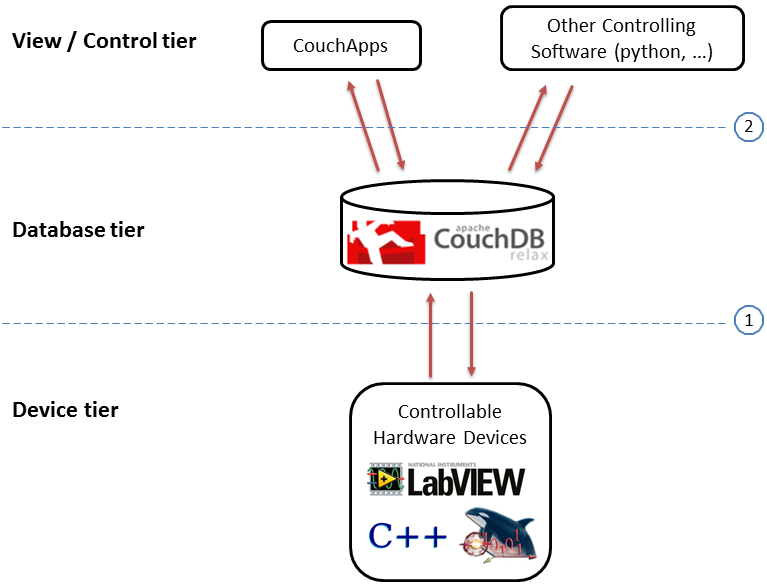
\includegraphics[width=0.7\textwidth]{images/ResultingFramework.png}
  \caption{Resulting framework for the nEDM experiment. Considering technical and conceptional aspects of necessary devices.}
  \label{figure:ResultingFramework}
\end{figure}

As shown in Figure \ref{figure:ResultingFramework}, the control and the device tier have to communicate with CouchDB. Therefore an API and a proper communication protocol has to be implemented. Two different interfaces exists regarding to the resulting framework:
\begin{itemize}
\item Between the device tier and the database tier (see Figure \ref{figure:ResultingFramework}: Interface 1)
\item Between the database tier and the view / control tier (see Figure \ref{figure:ResultingFramework}: Interface 2)
\end{itemize}
The communication between the view / control tier is easy, since so called CouchApps, small programs that are stored in the CouchDB and can access all data, are a built in functionality of CouchDB. They are mostly written in JavaScript and accessed via a web browser.\\
The interface between the device tier and the database is more sophisticated. Accessing CouchDB directly from LabVIEW is not possible and therefore an additional library is needed. This library is written in C (see Section \ref{section:implementation}). To ensure that this API allows different devices and sensors to send data to the database and receive data from it the functionality of the library has to be generic.

\subsection{Interfaces and communication between C and CouchDB}
Regarding to the resulting framework there exist two main interfaces (see Figure \ref{figure:ResultingFramework}). Whereas access the CouchDB via CouchApps is simple and easy to implement, accessing the database via C or C++ is not straightforward. Since it is possible to call C libraries from a LabVIEW solution, it is sufficient only to provide one platform independent library. Fortunately there is a platform independent library accessing CouchDB from any open-source project: pillowtalk \footnote{https://github.com/mgmarino/pillowtalk/}. This library uses libcurl and yajl to access CouchDB and communicates mainly via url targets. \\

\begin{figure}[h!]
  \centering
      \includegraphics[width=0.5\textwidth]{images/SendReceiveData.png}
  \caption{Bidirectional communication between hardware devices and the database}
  \label{figure:BidirectionalCommunication}
\end{figure}

Figure \ref{figure:BidirectionalCommunication} shows, that a bidirectional communication between the hardware devices should be possible. 
\begin{description}
     \item[Send Data] Every hardware device should be able to insert measured data into the database. This is crucial to every data acquisition system. An easy and generic way to insert is desirable. Different types of physical values are going to be stored. CouchDB is, unlike relational databases, document-based and without any given schema. Sending data, or data insert, is the basic operation and the pillowtalk library provides proper methods to perform the insertion of a new document. 
     \item[Receive Data] Hardware devices need be controllable. It should be possible to enable or disable them via the database or to send them commands to control their operations and set parameters. This functionality should be event based to avoid time and resource consuming polling tasks. 
\end{description}

To perform the bidirectional communication and to provide an interface to the functionality of pillowtalk a library called "AccCouchDB" \footnote{https://github.com/bwaltl/accCouchDB} was created. The library is platform independent and can be used on a Windows system or on Linux and Unix platforms. The library provides all functionality needed to insert data and to retrieve commands from the database. If a device wants to insert data, it is expected to register at the beginning at the database. This registration is necessary because later on, the CouchApp allows interaction only with registered devices. The registration process is quite easy since it consists only of one insertion with a fixed schema.

\begin{figure}[h!]
  \centering
      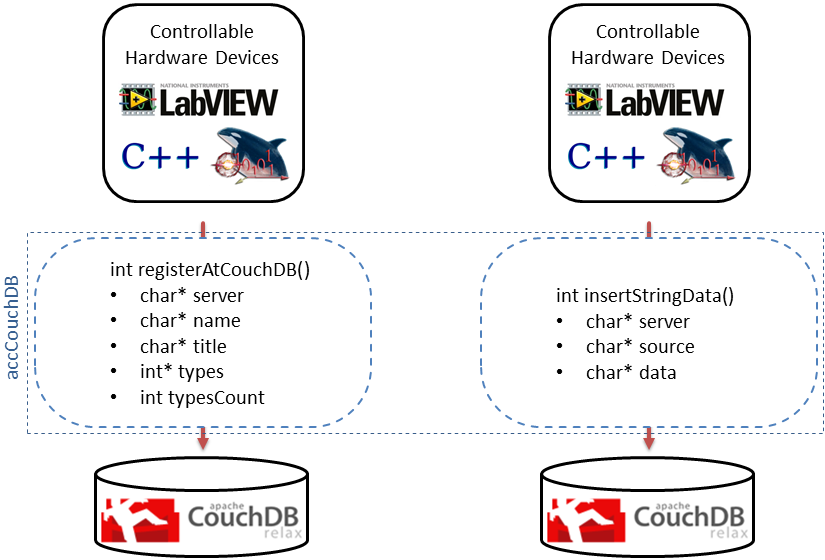
\includegraphics[width=0.7\textwidth]{images/SendingData2CouchDB.png}
  \caption{Inserting data at CouchDB}
  \label{figure:InsertingData}
\end{figure}

Figure \ref{figure:InsertingData} shows the two cases of a data insert operation. It is possible to register a device at CouchDB. This registration is done by calling a method named "registerAtCouchDB()":
\begin{description}
\item[char* server] The server parameter is used to connect to the database. It contains a string that holds the complete URL to the server and the database.
\item[char* name] The name parameter identifies the hardware device. This device name must be unique to ensure that it can be mapped correctly. 
\item[char* title] Since the name of a device must be unique within one database it is possible to define a more readable title to a hardware device. This must not be uniquely and allows a more detailed description of a device.
\item[int* types] A hardware device can be of a given type to enable aggregation or grouping at some view or controlling level. At the registration a device can specify to what types it belongs. Later on this could be mapped to, for instance, spatial or device type information.
\item[int typesCount] The number of types that a device belongs to. Length of the integer array "types".
\end{description}

Although it is not necessary, it may makes an implementation of a filter of notifications more convenient. This is more a preparation for further functionality, to develop some filtering functionality so that not every notification is passed to every device. \\

\begin{figure}[h!]
  \centering
      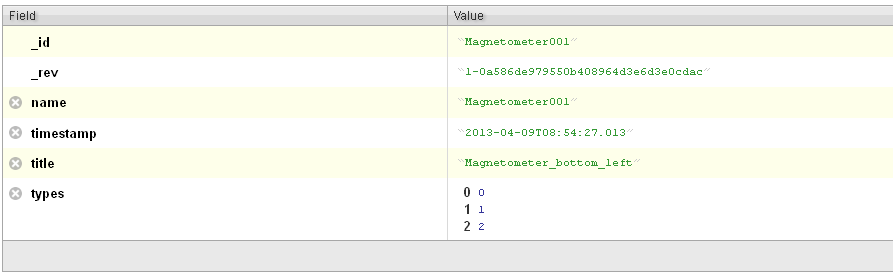
\includegraphics[width=0.9\textwidth]{images/CouchDBDoc_Register.png}
  \caption{CouchDB document format for a registered device}
  \label{figure:CouchDBDocumentFormat}
\end{figure}

Figure \ref{figure:CouchDBDocumentFormat} visualizes an inserted document at CouchDB. The id of the document is the name of the device, which is also contained in the "name" field. Also the "title" field is set to the value given by the function call. The types array contains three different values: 0,1,2. The "timestamp" field is set automatically by the accCouchDB library. \\

Figure \ref{figure:InsertingData} shows furthermore the data insert operation for measured data. This data insert is done calling the "insertStringData()":
\begin{description}
\item[char* server] The server parameter is used to connect to the database. It contains a string that holds the complete URL to the server and the database.
\item[char* source] The source parameter is used to map a data value to a device. The source string must match the "name" string that was specified by the registration of the device. 
\item[char* data] The data string contains the measured value of a physical phenomena. All data is stored as string values. 
\end{description}

Figure \ref{figure:CouchDBDocumentFormatData} shows an example of an inserted data document at CouchDB. The id of the document is the name of the device with a "data\_" prefix and an appended timestamp to ensure uniqueness. The "source" field is set to the value given by the function call that corresponds to the inserting device. The "data" field contains the measured value and the timestamp is added automatically.

\begin{figure}[h!]
  \centering
      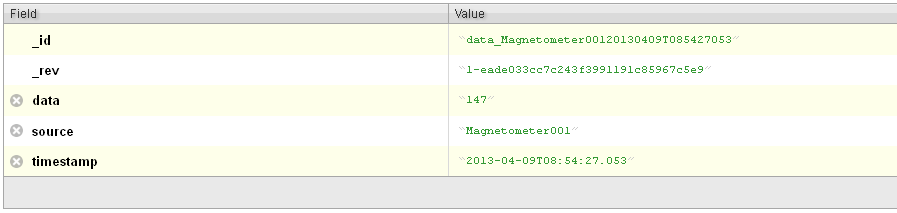
\includegraphics[width=0.9\textwidth]{images/CouchDBDoc_Data.png}
  \caption{CouchDB document format for measured data}
  \label{figure:CouchDBDocumentFormatData}
\end{figure}

\subsection{Retrieving commands and the CouchDB changes feed}
Enabling the possibility to turn on or off any functionality of the hardware device or to receive some other controlling commands it is necessary to communicate with the device. Since CouchDB supports notification services \footnote{http://guide.couchdb.org/draft/notifications.html} and the pillowtalk library also provides the functionality to use the changes feed it is not necessary for devices to poll if any commands are sent to them. Therefore there is a document type called "notification". \\

\begin{figure}[h!]
  \centering
      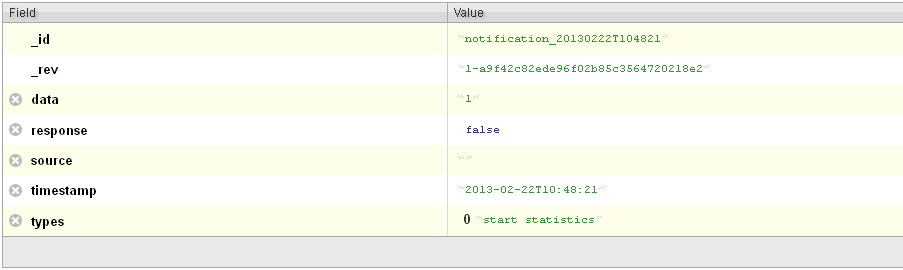
\includegraphics[width=0.9\textwidth]{images/CouchDBDoc_Notification.png}
  \caption{CouchDB document format for a notification}
  \label{figure:CouchDBDocumentFormatNotification}
\end{figure}

The notification document holds a data field of a value that is sent to the LabVIEW device. Furthermore it holds a response field that indicates if the transmission of the notification was successful. If not, the library creates a "error" field in the document in case of any error during the notification. This error field needs to be checked manually. It would be possible to implement further notification or logging in case of problems. Every command that will be sent to a device is stored in the database. Basically every controlling software is able to insert commands. \\

The notification is registered from the CouchDB with the changes feed functionality and is passed to LabVIEW using so called PostLVUserEvent \footnote{http://zone.ni.com/reference/en-XX/help/371361F-01/lvexcode/postlvuserevent/}. A LabVIEW VI can register to a changes feed of a CouchDB database and will be notified via callbacks on any changes or new documents. In principle only documents whose id field starts with "notification\_" will be passed. In more advanced applications additional filter methods will be required. This be implemented using the types field. To see how the notification process is implemented in LabVIEW see chapter \ref{section:implementation}.